
\documentclass[11pt]{amsbook}

\usepackage{../HBSuerDemir}	

\begin{document}


\hPage{b1p2/340}


	\begin{enumerate}
		\item[102.]Sketch the graph and determine the asymptotes if any of the following curve: $r = \frac{10}{2+3\cos0}$
		\item[103.]Find the polar form of $\frac{1+2i}{2+i}$ without performing the division.
		\item[104.]Compute $(\sqrt{3}+i)^6$
		\item[105.]Express the following in a simpler form:\\
		$1+\cos\theta+$.....$+\cos n\theta$,$\sin\theta+$......$+\sin n\theta.$  \\
	\end{enumerate}

	\begin{center}
		\title \text {ANSWERS TO EVEN NUMBERED EXERCISES}		
	\end{center}

	\begin{enumerate}
		\item[84.]	
			\begin{enumerate}[label=\alph*)]
				\item $44x^2+36xy+71y^2-268x-426y+719=0$
				\item $4x^2-20xy-11y^2+12x+6y+45=0$
				\item $9x^2-12xy+4y^2-36x+50y+49=0$
			\end{enumerate}
		\item[86.]
			\begin{enumerate}[label=\alph*)]
				\begin{multicols}{2}
				\item $a=15/4, b=3, c=9/4$
				\item $a=15/4, b=5, c=75/12$
				\end{multicols}
			\end{enumerate}
		\item[88.]$3x^2+3y^2+4x+2y-15=0$
		\item[90.]$x^2-y^2=0$
		\item[92.]$5xy+8x =0$
		\item[94.]
			\begin{enumerate}[label=\alph*)]
				\begin{multicols}{2}
					\item $r(3\cos\theta - 2\sin\theta)-9=0$
					\item $r^2(b^2\cos^2\theta+a^2\sin^2\theta)=a^2b^2$
				\end{multicols}
			\end{enumerate}
		\item[96.]$2xy-3x-2y=0;$   $ r=0, r\sin2\theta=3 \cos\theta+2\sin\theta.$
		\item[100.]
			\begin{enumerate}[label=\alph*)]
				\begin{multicols}{3}
					\item an ellipse $e=1/2$ $ p=3$,$ a=2$,$b=\sqrt3$
					\item a hyperbola $e=4/3$,$p=2$,$ a=\frac{24}{7}$,$b=\frac{8\sqrt7}{7}$
					\begin{flushleft}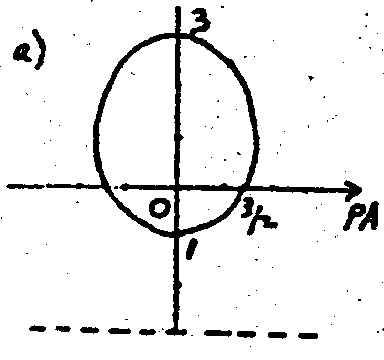
\includegraphics[width=0.25\textwidth,keepaspectratio=true]{images/b1p2-340-fig01}\end{flushleft}
					\begin{flushleft}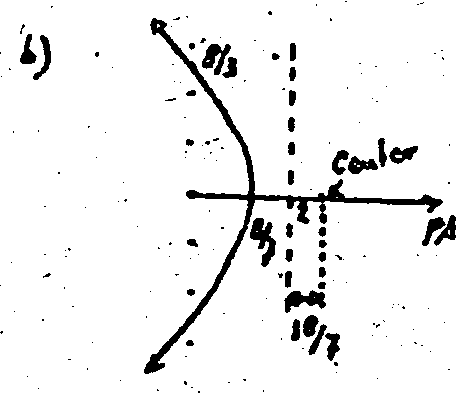
\includegraphics[width=0.25\textwidth,keepaspectratio=true]{images/b1p2-340-fig02}\end{flushleft}
				\end{multicols}
			\end{enumerate}
		\item[102.]  
			$ $
			\begin{multicols}{2}
				\begin{flushleft}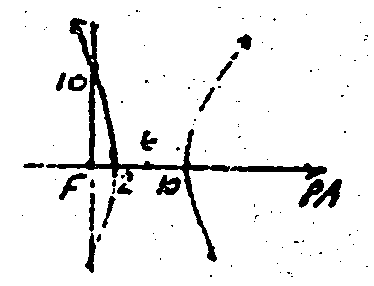
\includegraphics[width=0.4\textwidth,keepaspectratio=true]{images/b1p2-340-fig03}\end{flushleft}
				$r\cos[\theta-\arccos(-2/3)]-2\sqrt5=0$
			\end{multicols}
		\item[104.]-64
	\end{enumerate}
	
\end{document}  
